\documentclass[11pt,a4paper]{article}
\usepackage[utf8]{inputenc}
\usepackage[T1]{fontenc}
\usepackage[margin=2cm]{geometry}
\usepackage{graphicx}
\usepackage[table,svgnames]{xcolor}
\usepackage[many]{tcolorbox}
\usepackage{tikz}
\usetikzlibrary{shapes.geometric, arrows.meta, positioning, shadows, calc}
\usepackage{booktabs}
\usepackage{tabularx}
\usepackage{array}
\usepackage{amsmath,amssymb}
\usepackage{fancyhdr}
\usepackage{titlesec}
\usepackage{enumitem}
\usepackage{hyperref}
\usepackage{longtable}

\setlength{\headheight}{14pt}

% --- PALETA FRUTIGER AERO / XBOX 360 / GLASSMORPHISM ---
\definecolor{aerocyan}{RGB}{170, 220, 245}
\definecolor{aeromint}{RGB}{168, 230, 207}
\definecolor{aeropastelgreen}{RGB}{205, 245, 220}
\definecolor{aeroemerald}{RGB}{16, 172, 132}
\definecolor{aerolavender}{RGB}{225, 205, 245}
\definecolor{aerodark}{RGB}{35, 48, 60}
\definecolor{glassbg}{RGB}{247, 252, 255}
\definecolor{glassborder}{RGB}{185, 225, 245}
\definecolor{softpeach}{RGB}{255, 230, 220}
\definecolor{lavenderbg}{RGB}{247, 243, 253}

\hypersetup{
  colorlinks=true,
  linkcolor=aeroemerald,
  urlcolor=aeroemerald,
  citecolor=aeroemerald,
  pdftitle={WienerCalc -- Guia Oficial de Usuario},
  pdfauthor={WienerHoundStudios}
}

% --- ESTILO DE PÁGINA ---
\pagestyle{fancy}
\fancyhf{}
\rhead{\textcolor{aeroemerald}{\small\textbf{WienerCalc} --- Guía Oficial}}
\lhead{\textcolor{aerodark}{\small\textsf{WienerHoundStudios}}}
\rfoot{\textcolor{gray}{\small Página \thepage}}
\lfoot{\textcolor{gray}{\small Análisis Nutricional Universal}}
\renewcommand{\headrulewidth}{0.5pt}
\renewcommand{\footrulewidth}{0.4pt}

% --- FORMATO DE TÍTULOS ---
\titleformat{\section}
  {\color{aeroemerald}\normalfont\LARGE\bfseries}
  {\thesection}{1em}{}
  [\color{aerocyan}\rule{\linewidth}{1.5pt}]

\titleformat{\subsection}
  {\color{aerodark}\normalfont\Large\bfseries}
  {\thesubsection}{1em}{}

\titleformat{\subsubsection}
  {\color{aeroemerald}\normalfont\large\bfseries}
  {\thesubsubsection}{1em}{}

% --- CAJAS ESTILO GLASSMORPHISM (TCOLORBOX) ---
\newtcolorbox{glassbox}[1][]{
  enhanced,
  colback=glassbg,
  colframe=glassborder,
  arc=8pt,
  boxrule=1.2pt,
  shadow={2pt}{-2pt}{0pt}{black!12},
  fonttitle=\bfseries\color{aerodark},
  coltitle=aerodark,
  colbacktitle=aerocyan!40,
  title={#1},
  top=10pt,bottom=10pt,left=10pt,right=10pt,
  breakable
}

\newtcolorbox{tipbox}[1][]{
  enhanced,
  colback=aeropastelgreen!30,
  colframe=aeroemerald,
  colbacktitle=aeroemerald,
  arc=6pt,
  boxrule=1.5pt,
  leftrule=6pt,
  fonttitle=\bfseries\color{white},
  coltitle=white,
  title={CONSEJO: #1},
  top=8pt,bottom=8pt,left=10pt,right=10pt,
  breakable
}

\newtcolorbox{warningbox}[1][]{
  enhanced,
  colback=softpeach!40,
  colframe=OrangeRed!80,
  colbacktitle=OrangeRed!80,
  arc=6pt,
  boxrule=1.5pt,
  leftrule=6pt,
  fonttitle=\bfseries\color{white},
  coltitle=white,
  title={ATENCIÓN: #1},
  top=8pt,bottom=8pt,left=10pt,right=10pt,
  breakable
}

\newtcolorbox{faqbox}[1][]{
  enhanced,
  colback=lavenderbg,
  colframe=aerolavender,
  arc=6pt,
  boxrule=1.3pt,
  leftrule=5pt,
  fonttitle=\bfseries\color{aerodark},
  title={\textcolor{aeroemerald}{?} #1},
  top=8pt,bottom=8pt,left=10pt,right=10pt,
  breakable
}

\newtcolorbox{stepcard}[2][]{
  enhanced,
  colback=glassbg,
  colframe=aeromint,
  arc=8pt,
  boxrule=1.5pt,
  shadow={3pt}{-3pt}{0pt}{black!8},
  fonttitle=\bfseries\color{aerodark},
  colbacktitle=aeromint!50,
  title={#2},
  breakable,
  #1
}

\begin{document}

% ================= BANNER PRINCIPAL DE TÍTULO (FRUTIGER AERO VIBES) =================
\begin{center}
\begin{tikzpicture}
  \node[
    draw=glassborder,
    fill=glassbg,
    rounded corners=14pt,
    inner sep=14pt,
    line width=1.5pt,
    drop shadow={opacity=0.15, shadow xshift=3pt, shadow yshift=-3pt}
  ] (banner) {
    \begin{minipage}{0.94\textwidth}
      \begin{minipage}{\linewidth}
        \centering
        
\includegraphics[height=2.2cm]{images/logo.png} \\[6pt]
        {\Huge \bfseries \color{aeroemerald} WienerCalc} \\[4pt]
        {\large \bfseries \color{aerodark} Guía Oficial de Usuario} \\[2pt]
        {\small \color{gray} El motor universal para el análisis nutricional y evaluación de la ingesta} \\[6pt]
        \begin{tikzpicture}
          \shade[left color=aerocyan, right color=aeromint] (0,0) rectangle (12,0.08);
        \end{tikzpicture}
      \end{minipage}
    \end{minipage}

  };
\end{tikzpicture}
\end{center}

\vspace{0.3cm}

\begin{glassbox}[Bienvenido a WienerCalc]
Bienvenido a la guía completa de \textbf{WienerCalc}, el software profesional desarrollado por \textbf{WienerHoundStudios} para nutricionistas, epidemiólogos, investigadores, clínicas, universidades y profesionales de la salud.

WienerCalc traduce y moderniza la potencia del histórico algoritmo científico \textit{FoodCalc} en una interfaz gráfica rápida y elegante. Está diseñado para procesar desde pequeñas consultas nutricionales hasta masivas encuestas de salud poblacional con miles de pacientes.
\end{glassbox}

\vspace{0.3cm}

\renewcommand{\contentsname}{Índice de Contenidos}
\tableofcontents

\vspace{0.4cm}

% ================= SECCIÓN 1 =================
\section{Introducción y Filosofía del Software}

\textbf{WienerCalc} es una plataforma de procesamiento nutricional diseñada bajo una \textbf{arquitectura abierta y libre de restricciones}.

A diferencia de los programas tradicionales que encierran al usuario en bases de datos propietarias o fórmulas rígidas, WienerCalc se fundamenta en la \textbf{autonomía de los datos}:
\begin{itemize}[label=\textcolor{aeroemerald}{$\bullet$}]
    \item \textbf{Sin bloqueos de formato:} Trabaja directamente con tus propios archivos CSV de cualquier fuente o país.
    \item \textbf{Sin límites de columnas:} Soporta esquemas nutricionales de cualquier extensión o nivel de detalle.
    \item \textbf{Fórmulas dinámicas:} Permite definir reglas matemáticas personalizadas sin modificar el núcleo de la aplicación.
\end{itemize}

\vspace{0.4cm}

% ================= SECCIÓN 2 =================
\section{Alcance Real y Capacidades del Sistema}

WienerCalc es un procesador nutricional de alcance universal diseñado para adaptarse a cualquier flujo de trabajo:

\begin{glassbox}[1. Compatibilidad Universal con Tablas Nutricionales]
Funciona con cualquier tabla nacional o internacional existente (USDA, REDCA, TCAC, EuroFIR, Souci-Fachmann-Kraut, INCAP, LATINFOODS, \texttt{tpaisa.csv}, o tablas personalizadas).
\begin{itemize}[label=\textcolor{aeroemerald}{$\checkmark$}]
    \item \textbf{Nutrientes ilimitados:} Procesa simultáneamente calorías, macronutrientes, micronutrientes (vitaminas y minerales), ácidos grasos (saturados, mono y poliinsaturados), aminoácidos, fracciones de fibra (cruda, dietética, soluble, insoluble), cenizas, contenido de agua, índice glucémico, carga glucémica, etc.
\end{itemize}
\end{glassbox}

\vspace{0.3cm}

\begin{glassbox}[2. Motor Matemático de Fórmulas Personalizadas Ilimitado]
Te permite escribir \textbf{cualquier fórmula matemática} que requiera tu investigación o consulta médica usando cualquier combinación de columnas y unidades:
\begin{itemize}[label=\textcolor{aeroemerald}{$\checkmark$}]
    \item Cálculo de Energía en Kilocalorías ($\text{kcal}$) o Kilojulios ($\text{kJ}$).
    \item Porcentajes de distribución de macronutrientes (\% de calorías provenientes de grasas, proteínas o carbohidratos).
    \item Conversiones compuestas de Vitamina A (Retinol, Betacarotenos, UI, ER, RAE).
    \item Relaciones sodio/potasio, ratios de ácidos grasos (Omega-3/Omega-6), densidad de nutrientes por 1000 kcal, puntajes de calidad proteica, etc.
\end{itemize}
\end{glassbox}

\vspace{0.3cm}

\begin{glassbox}[3. Descomposición de Recetas, Cocción y Partes No Comestibles]
\begin{itemize}[label=\textcolor{aeroemerald}{$\checkmark$}]
    \item \textbf{Platos y recetas preparadas (fusionar):} Une tablas secundarias de preparaciones pre-calculadas (\texttt{trecetas.csv}) directamente a la tabla de alimentos.
    \item \textbf{Descomposición por ingredientes (diccionario):} Escala lotes enteros de recetas (\texttt{ejemreceta.csv}) recalculando proporcionalmente cada ingrediente bruto según la cantidad consumida.
    \item \textbf{Factores de Retención y Pérdida por Cocción:} Aplica porcentajes reales de retención/pérdida nutricional según el método de preparación (hervido, frito, horneado, asado, al vapor, microondas) sobre cualquier nutriente sensible (Vitamina C, complejo B, potasio, etc.).
    \item \textbf{Partes No Comestibles:} Deduce cáscaras, semillas, huesos o piel, calculando automáticamente el peso neto comestible real ingerido.
\end{itemize}
\end{glassbox}

\vspace{0.3cm}

\begin{glassbox}[4. Agrupación y Agregación Multinivel]
Agrupa y suma los resultados por \textbf{una o varias} columnas a la vez:
\begin{itemize}[label=\textcolor{aeroemerald}{$\checkmark$}]
    \item Paciente / sujeto de estudio (\texttt{id} / \texttt{person\_id}).
    \item Día de encuesta o seguimiento (\texttt{dia}).
    \item Tipo de comida (desayuno, almuerzo, cena, snack).
    \item Grupo poblacional, cohorte o municipio.
    \item O combinaciones: \textbf{sujeto + día}, \textbf{sujeto + tiempo de comida}, etc.
\end{itemize}
\end{glassbox}

\vspace{0.3cm}

\begin{glassbox}[5. Trazabilidad: nada se descarta en silencio]
Cada ejecución produce un \textbf{informe} con los avisos, las estadísticas y la lista de códigos que no se encontraron. Si un registro no entró en los totales, sabrás cuál, por qué y cuánta cantidad representaba. El informe se puede exportar en \texttt{.txt} para archivarlo junto a los resultados.
\end{glassbox}

\vspace{0.3cm}

\begin{glassbox}[6. Exportación Profesional y Compatible con Cualquier Software Estadístico]
Los resultados salen listos tanto para presentar como para analizar en masa:
\begin{itemize}[label=\textcolor{aeroemerald}{$\checkmark$}]
    \item \textbf{Excel (.xlsx) con formato real:} encabezado en color con texto en negrita, bordes, filas alternadas (``cebra''), ancho de columna ajustado al contenido, fila de encabezado congelada y autofiltro. Funciona igual en la aplicación de escritorio y en la versión web: los dos generan el mismo archivo \texttt{.xlsx}.
    \item \textbf{CSV listo para R, Python (pandas), SPSS, Stata o SAS:} sólo se entrecomilla lo que realmente lo necesita, y las columnas internas de WienerCalc (como \texttt{\_registros} o \texttt{\_cantidad\_total}) se renombran automáticamente al exportar para que R no las confunda con nombres inválidos. También protege contra ``CSV injection'': un valor de texto que empiece por \texttt{=}, \texttt{+}, \texttt{-} o \texttt{@} se neutraliza para que Excel o Sheets nunca lo interpreten como fórmula.
\end{itemize}
\end{glassbox}

\vspace{0.5cm}

% ================= SECCIÓN 3 =================
\section{Los 3 Archivos de Datos (Flexibilidad de Formato)}

WienerCalc utiliza archivos en formato estándar \textbf{CSV} (compatibles con Excel):

\begin{description}[font=\color{aeroemerald}\bfseries]
    \item[1. Tabla de Alimentos (Nutrientes) --- \textit{Obligatorio}] Tu base de datos nutricional de referencia con aportes expresados por cada \textbf{100 gramos}. Puede tener desde 3 columnas hasta más de 100.
    \item[2. Cantidades Consumidas (Entrada / Ingesta) --- \textit{Obligatorio}] El registro o encuesta alimentaria con lo consumido por los pacientes (códigos de alimentos, cantidades y, opcionalmente, métodos de cocción o momento del día).
    \item[3. Diccionario o Tabla de Recetas --- \textit{Opcional}] La lista de recetas compuestas o tabla de preparaciones secundarias que deseas integrar con la tabla principal.
\end{description}

\vspace{0.5cm}

% ================= SECCIÓN 4 =================
\section{Guía Paso a Paso por Pestañas}

El flujo de trabajo en WienerCalc está organizado en \textbf{4 Pestañas Secuenciales}:

\begin{center}
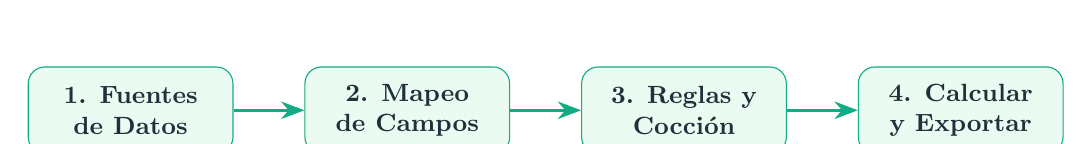
\begin{tikzpicture}[
  box/.style={draw=aeroemerald, fill=aeropastelgreen!40, rounded corners=6pt, minimum height=1.1cm, minimum width=2.6cm, align=center, font=\small\bfseries\color{aerodark}},
  arr/.style={-Stealth, aeroemerald, line width=1.2pt}
]
  \node[box] (p1) {1. Fuentes\\de Datos};
  \node[box, right=0.9cm of p1] (p2) {2. Mapeo\\de Campos};
  \node[box, right=0.9cm of p2] (p3) {3. Reglas y\\Cocción};
  \node[box, right=0.9cm of p3] (p4) {4. Calcular\\y Exportar};
  \draw[arr] (p1) -- (p2);
  \draw[arr] (p2) -- (p3);
  \draw[arr] (p3) -- (p4);
\end{tikzpicture}
\end{center}

\vspace{0.4cm}

\begin{stepcard}{Pestaña 1: Fuentes de Datos (Cargar CSVs)}
\begin{enumerate}[leftmargin=*]
    \item Haz clic en la primera caja morada \textbf{"Tabla de Alimentos (Nutrientes)"} para seleccionar tu base de datos (ej. \texttt{tpaisa.csv} o \texttt{foods.csv}).
    \item Haz clic en la segunda caja \textbf{"Cantidades Consumidas (Entrada)"} y selecciona tu archivo de ingesta (ej. \texttt{ejemingre.csv} u \texttt{input.csv}).
    \item \textit{(Opcional)} Si utilizas recetas compuestas, haz clic en la tercera caja \textbf{"Tabla de Recetas"} (ej. \texttt{trecetas.csv} o \texttt{ejemreceta.csv}).
\end{enumerate}

Al cargar cada archivo, debajo de la caja aparece un resumen de lo detectado: \textbf{número de filas, número de columnas y el delimitador}. Conviene mirarlo: si el delimitador no es el que esperabas, probablemente el archivo se guardó con otra configuración regional.

\begin{tipbox}[Quitar o reemplazar un archivo]
Cada caja con un archivo cargado muestra una \textbf{×} en su esquina superior derecha. Al pulsarla se retira el archivo, se limpian las selecciones que dependían de él (columnas, alias, reglas de cocción) y se descartan los resultados anteriores, porque ya no corresponden a la configuración actual. También puedes simplemente hacer clic en la caja para reemplazar el archivo por otro.
\end{tipbox}

\begin{glassbox}[Modo de la Tabla de Recetas]
Al cargar el tercer archivo aparece un selector con tres opciones. \textbf{Elegir bien esto es importante:} dos archivos con la misma pinta pueden significar cosas distintas.
\begin{itemize}[label=\textcolor{aeroemerald}{$\rightarrow$}]
    \item \textbf{Preparaciones precalculadas (fusionar):} cada fila es un plato ya calculado (con sus nutrientes por 100\,g) que se incorpora a la tabla de alimentos. Es el caso de \texttt{trecetas.csv}.
    \item \textbf{Diccionario de ingredientes (descomponer):} cada fila es \textbf{un ingrediente} de una receta. WienerCalc descompone la receta y escala cada ingrediente en proporción a la cantidad consumida. En este modo debes indicar tres columnas: receta, ingrediente y cantidad.
    \item \textbf{Detectar automáticamente:} WienerCalc decide y \textbf{te dice qué eligió} en el informe de la ejecución. Si el archivo es ambiguo, lo advierte en vez de asumir.
\end{itemize}
\end{glassbox}

\begin{warningbox}[Si un código existe en AMBAS tablas]
Cuando un mismo código aparece en la tabla de alimentos y en la de preparaciones, hay que decidir cuál manda. WienerCalc te lo pregunta y \textbf{te informa cuántos códigos colisionaron}.

Esta elección \textbf{cambia tus resultados}: en el dataset \texttt{tpaisa} + \texttt{trecetas} colisionan 52 códigos, y la diferencia en grasa total del sujeto de prueba es del 123\,\%. Ninguna de las dos opciones es ``la correcta'' en abstracto: depende de si en tu estudio esos códigos representan el alimento crudo o la preparación. Lo que sí es incorrecto es resolverlo sin saberlo.
\end{warningbox}
\end{stepcard}

\vspace{0.4cm}

\begin{stepcard}{Pestaña 2: Mapeo de Campos, Agrupación y Alias}
En esta pestaña defines la estructura de tus archivos:
\begin{enumerate}[leftmargin=*]
    \item \textbf{Columna ID (Tabla Alimentos):} Selecciona el código de alimento (ej. \texttt{codalim} o \texttt{food\_id}).
    \item \textbf{Columna ID (Consumo Entrada):} Selecciona el código en la tabla de ingesta (ej. \texttt{codalim} u \texttt{input\_id}).
    \item \textbf{Nombre de Columna de Cantidad:} Selecciona la columna de peso (ej. \texttt{cantidad} u \texttt{amount\_grams}).
    \item \textbf{Escala de Entrada (Multiplicador):} escribe \textbf{\texttt{0.01}} si tus datos de consumo están en \textbf{gramos} ($150\,\text{g} \times 0.01 = 1.5\,\text{porciones de 100g}$), o \textbf{\texttt{1.0}} si ya vienen en porciones de 100\,g. El campo se pone rojo si el valor no es un número mayor que 0.
    \item \textbf{Columna de Método de Cocción (Opcional):} Selecciona la columna que indica el tipo de cocción (ej. \texttt{tipocomi} o \texttt{prep\_method}).
    \item \textbf{Columna de Parte No Comestible (Opcional):} Selecciona la columna con el factor de desecho e indica si está expresada como \textbf{fracción (0--1)} o \textbf{porcentaje (0--100)}. Si el valor no encaja con la unidad elegida, WienerCalc lo avisa en vez de anular los nutrientes de ese alimento.
    \item \textbf{Agrupar Resultados Por (Opcional):} Marca \textbf{una o varias} columnas. Con \texttt{id} obtienes una fila por sujeto; con \texttt{id} \textbf{y} \texttt{dia} obtienes una fila por sujeto y día.
\end{enumerate}

\begin{glassbox}[Columnas Descriptivas (nunca se suman)]
Marca aquí las columnas que son numéricas pero \textbf{no son nutrientes}: \texttt{orden}, \texttt{dia}, \texttt{tipocomi}, códigos, identificadores. Si no lo haces, al agrupar se sumarían como si fueran nutrientes. WienerCalc preselecciona automáticamente los nombres más habituales que encuentre en tus archivos, pero conviene revisarlo.
\end{glassbox}

\begin{glassbox}[Alias de Columnas (Unir Recetas y Alimentos)]
Si tu tabla de recetas utiliza nombres de columnas distintos a la tabla principal, empareja los campos usando el botón \textbf{"+ Añadir Alias"}:
\begin{center}
\begin{tabular}{@{}ll@{}}
\toprule
\textbf{Col. Recetas (\texttt{trecetas.csv})} & \textbf{Col. Alimentos (\texttt{tpaisa.csv})} \\
\midrule
\texttt{cod\_b} & \texttt{codalim} \\
\texttt{Kcal} & \texttt{kcal} \\
\texttt{Pro. g.} & \texttt{proteina\_g} \\
\texttt{GT. g.} & \texttt{grasatot\_g} \\
\texttt{CHO. g.} & \texttt{Carboh\_g} \\
\texttt{VA (UI)} & \texttt{vitaA(UI)} \\
\texttt{VA (ER)} & \texttt{vitaA(ER)} \\
\bottomrule
\end{tabular}
\end{center}
\end{glassbox}
\end{stepcard}

\vspace{0.4cm}

\begin{stepcard}{Pestaña 3: Reglas Matemáticas e Impacto de Cocción}

\subsubsection*{1. Reglas Matemáticas Personalizadas (Fórmulas Ilimitadas)}
Haz clic en \textbf{"+ Añadir Regla"} para definir cualquier ecuación. El editor de fórmulas está pensado para que armar una ecuación compleja no se sienta como escribir código a ciegas:

\begin{itemize}[label=\textcolor{aeroemerald}{$\checkmark$}]
    \item \textbf{Variables clicables:} haz clic sobre cualquier columna disponible y se inserta \textbf{directamente en la posición del cursor} dentro de la fórmula (no hay que copiar y pegar).
    \item \textbf{Paréntesis con colores por nivel (``rainbow parens''):} cada nivel de anidamiento se pinta de un color distinto, y un paréntesis sin pareja se marca en rojo al instante. Así se ve de un vistazo si \texttt{((a+b)*(c-d))/(e+f)} está bien armado.
    \item \textbf{Autocompletado de paréntesis:} al escribir \texttt{(} se inserta automáticamente su \texttt{)} de cierre con el cursor en medio; si ya hay un \texttt{)} justo después del cursor y vuelves a escribirlo, el editor pasa por encima en vez de duplicarlo; y borrar con retroceso un par recién abierto y vacío borra los dos caracteres juntos.
    \item \textbf{Barra de operadores:} botones para insertar \texttt{( )}, \texttt{+}, \texttt{-}, \texttt{×}, \texttt{÷}, \texttt{\^{}} y \texttt{,} directamente en el cursor.
    \item \textbf{Vista previa en vivo:} debajo de la fórmula se muestra el resultado calculado con \textbf{la primera fila real} de tu tabla de alimentos, para confirmar el número esperado antes de calcular sobre todos tus datos.
    \item \textbf{Galería de plantillas:} fórmulas nutricionales comunes ya armadas (energía Atwater en kcal y kJ, \% de energía por macronutriente, densidad de nutrientes por 1000 kcal, relación sodio/potasio) para insertar con un clic y ajustar a tus columnas.
\end{itemize}

Ejemplos de reglas típicas:
\begin{itemize}
    \item \textbf{Calorías de Grasas:} Campo: \texttt{cal\_from\_fat} $\rightarrow$ Fórmula: \texttt{grasatot\_g * 9}
    \item \textbf{Suma de Vitamina A:} Campo: \texttt{vitA\_sum} $\rightarrow$ Fórmula: \texttt{vitaA(UI) + vitaA(ER)}
    \item \textbf{Energía en Kilojulios (kJ):} Campo: \texttt{energia\_kJ} $\rightarrow$ Fórmula: \texttt{17 * proteina\_g + 38 * grasatot\_g + 17 * Carboh\_g}
    \item \textbf{Porcentaje de Energía de Proteínas:} Campo: \texttt{pct\_proteina} $\rightarrow$ Fórmula: \texttt{(proteina\_g * 4 / kcal) * 100}
\end{itemize}

\begin{tipbox}[Validación en vivo]
Mientras escribes, WienerCalc comprueba la fórmula contra las columnas de tus archivos. Si te equivocas en un nombre, el campo se pone rojo y sugiere la columna correcta (\textit{``Variable no encontrada: «proteina» (¿querías decir «protein»?)''}). Si el problema son los paréntesis, el mensaje lo dice de forma específica (\textit{``Falta cerrar un paréntesis''}, \textit{``Hay un paréntesis de cierre de más''}) en vez de un genérico error de sintaxis. Una fórmula inválida \textbf{deja la celda vacía}, nunca en \texttt{0}: un cero silencioso se confunde con un dato real.

\textbf{Funciones disponibles:} \texttt{min, max, abs, round, floor, ceil, sqrt, pow, ln, log, exp, if}. Operadores: \texttt{+ - * / \% \^{}}, paréntesis anidados sin límite de profundidad, comparaciones (\texttt{< > <= >= == !=}) y \texttt{\&\&} / \texttt{||}.
\end{tipbox}

\subsubsection*{2. Reducciones y Pérdidas por Cocción}
Haz clic en \textbf{"+ Añadir Regla de Cocción"} para descontar pérdidas de nutrientes sensibles:
\begin{itemize}
    \item \textbf{Método:} \texttt{boil} (hervido) o \texttt{fry} (frito).
    \item \textbf{Campo de Reducción:} \texttt{boil\_loss} (se acepta tanto \texttt{0.40} como \texttt{40} para un 40\,\% de pérdida).
    \item \textbf{Nutrientes Objetivo:} marca los nutrientes afectados (ej. \texttt{vitaC}, \texttt{vitaB1}, \texttt{potasio\_mg}).
\end{itemize}
\end{stepcard}

\vspace{0.4cm}

\begin{stepcard}{Pestaña 4: Calcular, Vista Previa y Exportación}
\begin{enumerate}[leftmargin=*]
    \item Haz clic en el botón \textbf{"Ejecutar Cálculo"} (Run Calculation).
    \item El motor procesará la combinación de tablas, recetas, agrupaciones y reglas matemáticas.
    \item Revisa los cinco indicadores: \textbf{alimentos cargados, recetas, registros leídos, filas de resultado y colisiones de códigos}. Si alguno no cuadra con lo que esperas, ahí está el problema.
    \item Lee el \textbf{Informe de la ejecución}, la parte más importante de esta pestaña:
    \begin{itemize}
        \item \textcolor{OrangeRed}{\textbf{Errores}} --- algo impidió calcular una regla.
        \item \textcolor{orange}{\textbf{Advertencias}} --- colisiones de códigos, filas mal formadas, cantidades vacías, columnas ausentes en una fórmula.
        \item \textcolor{aeroemerald}{\textbf{Información}} --- qué modo de receta se usó, cuántas preparaciones se incorporaron.
    \end{itemize}
    Si todo fue bien, verás en verde \textit{``Sin advertencias: todos los registros se procesaron.''}
    \item Revisa el panel \textbf{«Códigos que no existen en la tabla de alimentos»}, si aparece: lista cada código ausente, en cuántos registros aparecía y qué cantidad total quedó fuera del cálculo. \textbf{Esos registros no están sumados en tus totales.}
    \item Revisa la \textbf{Vista Previa de Resultados} (con desplazamiento horizontal).
    \item Exporta tu trabajo:
    \begin{itemize}[label=\textcolor{aeroemerald}{$\rightarrow$}]
        \item \textbf{Excel (.xlsx):} libro con encabezado en color y negrita, bordes, filas en cebra, columnas con ancho ajustado, fila de encabezado congelada y autofiltro --- \textbf{igual en la aplicación de escritorio y en la versión web}, ambas generan el mismo archivo.
        \item \textbf{CSV:} listo para SPSS, R, Stata, SAS o Python (pandas). Incluye BOM para que Excel respete los acentos al abrirlo directo, y sólo entrecomilla lo que realmente lo necesita.
        \item \textbf{Informe (.txt):} la configuración usada, las estadísticas, todos los avisos y la lista completa de códigos no encontrados. \textbf{Guárdalo junto a tus resultados:} documenta cómo se obtuvieron.
    \end{itemize}
\end{enumerate}

\begin{tipbox}[Abrir el CSV en Python o R]
Si vas a abrir el CSV con \texttt{pandas} en Python, usa \texttt{pd.read\_csv(archivo, encoding='utf-8-sig')} para que el BOM no se pegue al nombre de la primera columna. Con R (\texttt{read.csv} o \texttt{readr::read\_csv}) no hace falta nada especial.
\end{tipbox}

\begin{glassbox}[Columnas que añade WienerCalc a los resultados]
\begin{tabularx}{\linewidth}{@{}>{\raggedright\arraybackslash}p{2.6cm} >{\raggedright\arraybackslash}p{3.1cm} X@{}}
\toprule
\textbf{En pantalla} & \textbf{Al exportar a CSV} & \textbf{Significado} \\
\midrule
\texttt{\_registros} & \texttt{registros} & Cuántos registros se agregaron en esa fila \\[2pt]
\texttt{\_cantidad\_total} & \texttt{cantidad\_total} & Suma de las cantidades consumidas \\[2pt]
\texttt{\_porcion} & \texttt{porcion} & Suma de porciones (cantidad × escala × parte comestible) \\[2pt]
\texttt{primer\_<col>} & \textit{(sin cambio)} & Valor de una columna descriptiva no constante en el grupo \\
\bottomrule
\end{tabularx}
\vspace{4pt}
Las columnas que empiezan con \texttt{\_} sólo se ven así \textbf{dentro de la aplicación} (y en el .xlsx). Al exportar a \textbf{CSV} se les quita el guion bajo inicial, porque R convierte automáticamente cualquier cabecera que empiece por \texttt{\_} en algo como \texttt{X\_registros} al leerla con \texttt{read.csv()} --- quitarlo de antemano evita esa sorpresa. Las columnas de nutrientes que vienen de tu propia tabla de alimentos nunca se tocan, aunque tengan paréntesis o puntos en el nombre (como \texttt{vitaA(UI)}), porque renombrarlas rompería la referencia a tu tabla de composición original.
\end{glassbox}
\end{stepcard}

\vspace{0.5cm}

% ================= SECCIÓN 5 =================
\section{Gestión de Perfiles Reutilizables (.json)}

Para investigaciones continuas o consultas clínicas diarias, no necesitas volver a configurar columnas ni escribir fórmulas cada vez:
\begin{itemize}[label=\textcolor{aeroemerald}{$\bullet$}]
    \item \textbf{Guardar Perfil (Save Config):} Descarga un archivo \texttt{.json} con toda tu configuración (mapeos, alias, reglas, factores de cocción, agrupaciones, modo de receta y política de colisión).
    \item \textbf{Cargar Perfil (Load Config):} Restaura al instante toda tu configuración guardada con un solo clic.
\end{itemize}

\begin{tipbox}[Los perfiles antiguos siguen funcionando]
Los perfiles guardados con versiones anteriores se \textbf{migran automáticamente} al cargarlos (por ejemplo, la antigua agrupación por una sola columna pasa a la nueva lista de columnas).
\end{tipbox}

\vspace{0.3cm}

% ================= SECCIÓN 6 =================
\section{Editor de CSV / Terminal Integrado}

WienerCalc incluye un \textbf{Editor e Inspector de CSV en vivo} accesible desde cualquier pestaña:
\begin{enumerate}[leftmargin=*]
    \item Haz clic en el botón \textbf{\texttt{OPEN TERMINAL}} en la esquina superior derecha.
    \item Explora las pestañas de tus archivos (\texttt{foods.csv}, \texttt{input.csv}, \texttt{recipes.csv}).
    \item Verifica encabezados y valores en tiempo real, busca (\texttt{Ctrl + F}), reemplaza (\texttt{Ctrl + H}) y guarda ediciones directamente (\texttt{Ctrl + S}).
\end{enumerate}

\vspace{0.5cm}

% ================= SECCIÓN 7 =================
\section{Preguntas Frecuentes (FAQ) y Casos Prácticos}

\begin{faqbox}[¿WienerCalc viene con nutrientes bloqueados o rígidos?]
\textbf{No.} WienerCalc es 100\,\% dinámico. Si tu tabla de alimentos tiene 5 nutrientes o 120 (incluyendo antioxidantes, polifenoles o minerales traza), el motor procesará y calculará absolutamente todos.
\end{faqbox}

\vspace{0.3cm}

\begin{tipbox}[¿Por qué usamos la escala 0.01 para consumos en gramos?]
Las tablas nutricionales expresan los nutrientes por cada \textbf{100 gramos} de alimento.
Si un paciente consume \textbf{150 gramos}:
$$\text{Porciones} = 150\,\text{g} \times 0.01 = 1.5\,\text{porciones de 100g}$$
El motor multiplicará los nutrientes por $1.5$. Si tus registros están en kilogramos, la escala sería \texttt{10}. Si ya están en porciones de 100g, la escala es \texttt{1.0}.
\end{tipbox}

\vspace{0.3cm}

\begin{faqbox}[¿Qué formatos de CSV acepta?]
Todos los habituales, y los detecta solo:
\begin{itemize}[label=\textcolor{aeroemerald}{$\checkmark$}]
    \item \textbf{Delimitador:} coma, punto y coma, tabulador o barra vertical.
    \item \textbf{BOM UTF-8:} el «CSV UTF-8 (delimitado por comas)» que exporta Excel funciona sin más.
    \item \textbf{Campos entrecomillados:} un nombre como \texttt{"Arroz, blanco, cocido"} no rompe la fila.
    \item \textbf{Coma decimal:} \texttt{31,5} se interpreta como 31.5. También \texttt{1.234,56} y \texttt{1,234.56}.
    \item \textbf{Finales de línea:} Windows (CRLF), Unix (LF) o Mac clásico (CR).
    \item \textbf{Códigos:} se toleran los \texttt{101.0} que genera Excel al tratar los códigos como números, y los ceros a la izquierda se respetan.
\end{itemize}
Si dos columnas tienen el mismo nombre, la segunda se renombra (\texttt{a}, \texttt{a\_2}) en vez de sobrescribir a la primera en silencio.
\end{faqbox}

\vspace{0.3cm}

\begin{warningbox}[¿Qué pasa si un código de mi encuesta no está en la tabla de alimentos?]
Ese registro \textbf{no se suma} (no hay datos con los que sumarlo) y WienerCalc te lo dice explícitamente: aparece en el panel «Códigos que no existen en la tabla de alimentos» con el número de registros y la cantidad total afectada, y queda registrado en el informe \texttt{.txt}. Nunca desaparece en silencio.
\end{warningbox}

\vspace{0.3cm}

\begin{faqbox}[¿Los resultados de la versión web y la de escritorio son los mismos?]
\textbf{Sí, exactamente los mismos.} Ambas usan el mismo motor de cálculo; lo único que cambia es cómo se leen los archivos (el explorador del sistema frente al selector del navegador). La suite de pruebas del proyecto verifica esta igualdad en cada cambio, e incluye ambos formatos de exportación (CSV y Excel).

Diferencias que sí existen, y sólo de entrada/salida:
\begin{itemize}
    \item En la web los archivos viven en la memoria de la pestaña: si recargas la página, hay que volver a seleccionarlos, y las ediciones del terminal integrado no se escriben en tu disco.
    \item La exportación a Excel de la web usa la compresión propia del navegador (\texttt{CompressionStream}); en un navegador muy antiguo que no la soporte, verás un aviso claro en vez de un archivo dañado.
\end{itemize}
\end{faqbox}

\vspace{0.3cm}

\begin{faqbox}[¿Puedo abrir los resultados en R o Python (pandas) sin problemas?]
Sí. El CSV exportado sigue el formato que ambos leen por defecto: separador de coma, comillas sólo donde hacen falta, y el punto siempre como separador decimal (nunca coma), sin importar el idioma de tu computadora. Dos detalles a tener en cuenta:
\begin{itemize}
    \item Las columnas internas de WienerCalc (\texttt{\_registros}, \texttt{\_cantidad\_total}, \texttt{\_porcion}, \texttt{\_codigo}, \texttt{\_origen}) se exportan \textbf{sin el guion bajo inicial} (\texttt{registros}, \texttt{cantidad\_total}\ldots) para que R no las renombre solo.
    \item El archivo incluye BOM (para que Excel muestre bien los acentos al abrirlo directo). Con \texttt{pandas.read\_csv()} usa \texttt{encoding='utf-8-sig'}; con R no necesitas hacer nada especial.
\end{itemize}
\end{faqbox}

\vspace{0.3cm}

\begin{tipbox}[Diferencia entre Energía en Kilocalorías vs Kilojulios]
\begin{itemize}
    \item \textbf{Kilocalorías (kcal):} $4 \times \text{Proteínas} + 9 \times \text{Grasas} + 4 \times \text{Carbohidratos}$
    \item \textbf{Kilojulios (kJ):} $17 \times \text{Proteínas} + 38 \times \text{Grasas} + 17 \times \text{Carbohidratos}$
    \textit{Factores convertidos por la constante $1\,\text{kcal} = 4.184\,\text{kJ}$.}
\end{itemize}
\end{tipbox}

\vspace{0.6cm}

\begin{center}
\textcolor{gray}{\small --- Guía Oficial de Usuario WienerCalc | Desarrollado por WienerHoundStudios ---}
\end{center}

\end{document}
